\documentclass[border=10pt]{standalone}
\usepackage{ctex}
\usepackage{amsmath,amssymb,bm}
\usepackage{tikz}
\usepackage{tikz-feynman}
\tikzfeynmanset{compat=1.1.0}
\usetikzlibrary{positioning,arrows.meta,shapes.geometric,fit,backgrounds,calc}

% Smartart-style box
\tikzset{
  levelbox/.style={
    draw=#1, fill=#1!8, rounded corners=6pt,
    minimum width=5.5cm, minimum height=1.2cm,
    align=center, font=\small, inner sep=6pt
  },
  levelbox/.default=blue,
  arrowlabel/.style={font=\scriptsize\itshape, text=gray!70!black, midway},
  integralvar/.style={font=\scriptsize\ttfamily, text=red!80!black},
  feynbox/.style={draw=green!60!black, fill=green!5, rounded corners=4pt, inner sep=4pt},
}

\begin{document}
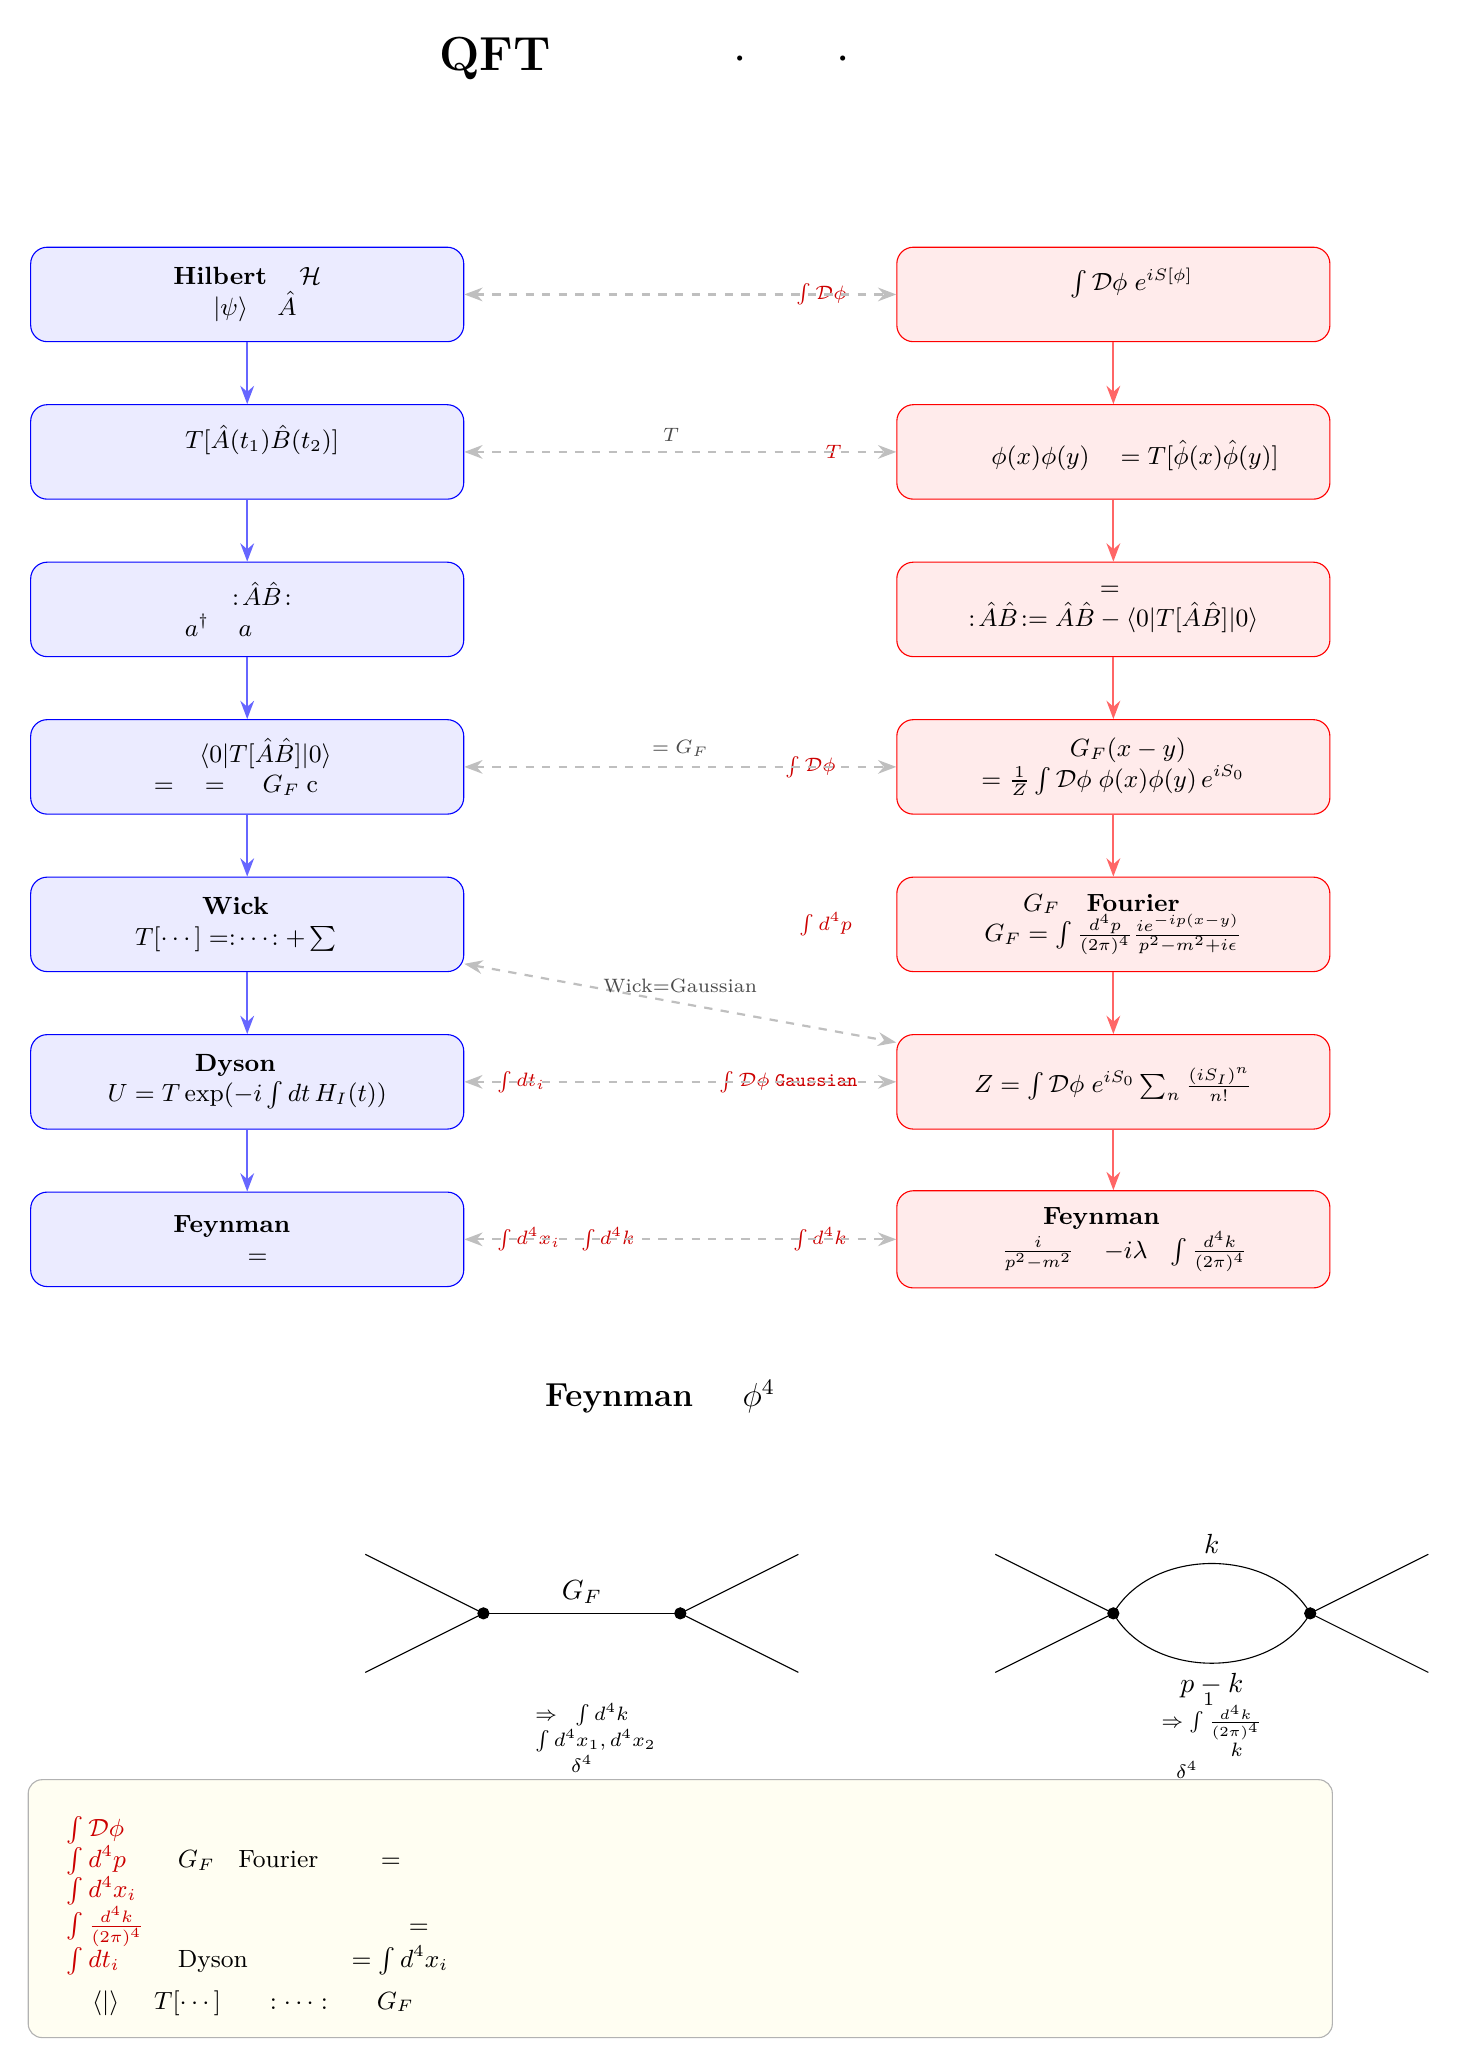
\begin{tikzpicture}[node distance=1.8cm and 2cm]

% ============================================================
% TITLE
% ============================================================
\node[font=\LARGE\bfseries] (title) at (0, 0) {QFT 微扰论的层级展开：符号 $\cdot$ 积分变量 $\cdot$ 物理含义};

% ============================================================
% LEFT COLUMN: Operator Language Hierarchy
% ============================================================
\node[font=\large\bfseries, text=blue!80!black] (op_title) at (-5.5, -1.5) {算符语言};

\node[levelbox=blue] (L0) at (-5.5, -3) {%
  \textbf{Hilbert 空间} $\mathcal{H}$\\
  态 $\vert\psi\rangle$，算符 $\hat{A}$
};
\node[integralvar, right=0.3cm of L0] {无积分};

\node[levelbox=blue] (L1) at (-5.5, -5) {%
  \textbf{编时积} $T[\hat{A}(t_1)\hat{B}(t_2)]$\\
  按时间重排算符（纯代数）
};
\node[integralvar, right=0.3cm of L1] {无积分};

\node[levelbox=blue] (L2) at (-5.5, -7) {%
  \textbf{正规序} $:\!\hat{A}\hat{B}\!:$\\
  $a^\dagger$ 全左，$a$ 全右（纯代数）
};
\node[integralvar, right=0.3cm of L2] {无积分};

\node[levelbox=blue] (L3) at (-5.5, -9) {%
  \textbf{真空期望} $\langle 0\vert T[\hat{A}\hat{B}]\vert 0\rangle$\\
  $=$ 收缩 $=$ 传播子 $G_F$（c 数）
};
\node[integralvar, right=0.3cm of L3] {无积分\\（结果）};

\node[levelbox=blue] (L4) at (-5.5, -11) {%
  \textbf{Wick 定理}\\
  $T[\cdots] = :\!\cdots\!: + \sum$ 收缩
};
\node[integralvar, right=0.3cm of L4] {无积分\\（恒等式）};

\node[levelbox=blue] (L5) at (-5.5, -13) {%
  \textbf{Dyson 级数}\\
  $U = T\exp(-i\int dt\,H_I(t))$
};
\node[integralvar, right=0.3cm of L5] {$\int dt_i$\\顶点时间};

\node[levelbox=blue] (L6) at (-5.5, -15) {%
  \textbf{Feynman 图求和}\\
  每个完全收缩 $=$ 一个图
};
\node[integralvar, right=0.3cm of L6] {$\int d^4x_i$ 顶点\\$\int d^4k$ 圈};

% Arrows left column
\foreach \a/\b in {L0/L1, L1/L2, L2/L3, L3/L4, L4/L5, L5/L6} {
  \draw[-{Stealth}, blue!60, thick] (\a) -- (\b);
}

% ============================================================
% RIGHT COLUMN: Path Integral Language
% ============================================================
\node[font=\large\bfseries, text=red!80!black] (pi_title) at (5.5, -1.5) {路径积分语言};

\node[levelbox=red] (R0) at (5.5, -3) {%
  \textbf{泛函积分} $\int\mathcal{D}\phi\;e^{iS[\phi]}$\\
  对所有场构型求和
};
\node[integralvar, left=0.3cm of R0] {$\int\mathcal{D}\phi$\\场构型};

\node[levelbox=red] (R1) at (5.5, -5) {%
  \textbf{自动编时}\\
  路径积分中 $\phi(x)\phi(y)$ 自动 $= T[\hat\phi(x)\hat\phi(y)]$
};
\node[integralvar, left=0.3cm of R1] {$T$ 消失};

\node[levelbox=red] (R2) at (5.5, -7) {%
  \textbf{正规序 $=$ 减去收缩}\\
  $:\!\hat{A}\hat{B}\!: = \hat{A}\hat{B} - \langle 0\vert T[\hat{A}\hat{B}]\vert 0\rangle$
};
\node[integralvar, left=0.3cm of R2] {代数};

\node[levelbox=red] (R3) at (5.5, -9) {%
  \textbf{传播子} $G_F(x-y)$\\
  $= \frac{1}{Z}\int\mathcal{D}\phi\;\phi(x)\phi(y)\,e^{iS_0}$
};
\node[integralvar, left=0.3cm of R3] {$\int\mathcal{D}\phi$\\（已积完）};

\node[levelbox=red] (R4) at (5.5, -11) {%
  \textbf{$G_F$ 的 Fourier 表示}\\
  $G_F = \int\frac{d^4p}{(2\pi)^4}\frac{ie^{-ip(x-y)}}{p^2-m^2+i\epsilon}$
};
\node[integralvar, left=0.3cm of R4] {$\int d^4p$\\动量};

\node[levelbox=red] (R5) at (5.5, -13) {%
  \textbf{微扰展开}\\
  $Z = \int\mathcal{D}\phi\;e^{iS_0}\sum_n\frac{(iS_I)^n}{n!}$
};
\node[integralvar, left=0.3cm of R5] {$\int\mathcal{D}\phi$\\（Gaussian）};

\node[levelbox=red] (R6) at (5.5, -15) {%
  \textbf{Feynman 规则}\\
  内线 $\frac{i}{p^2-m^2}$，顶点 $-i\lambda$，圈 $\int\frac{d^4k}{(2\pi)^4}$
};
\node[integralvar, left=0.3cm of R6] {$\int d^4k$\\圈动量};

% Arrows right column
\foreach \a/\b in {R0/R1, R1/R2, R2/R3, R3/R4, R4/R5, R5/R6} {
  \draw[-{Stealth}, red!60, thick] (\a) -- (\b);
}

% ============================================================
% HORIZONTAL ARROWS: equivalence
% ============================================================
\foreach \a/\b/\label in {L0/R0/定义等价, L1/R1/$T$ 自动, L3/R3/$=G_F$, L4/R5/Wick$=$Gaussian, L5/R5/展开, L6/R6/规则} {
  \draw[{Stealth}-{Stealth}, gray!50, dashed, thick] (\a) -- node[above, font=\scriptsize, text=gray!60!black] {\label} (\b);
}

% ============================================================
% BOTTOM: Feynman diagram examples
% ============================================================
\node[font=\large\bfseries] (feyn_title) at (0, -17) {Feynman 图示例（$\phi^4$ 理论）};

% Tree diagram
\begin{feynman}
  \vertex (i1) at (-4, -19);
  \vertex (i2) at (-4, -20.5);
  \vertex (v1) at (-2.5, -19.75);
  \vertex (v2) at (0, -19.75);
  \vertex (o1) at (1.5, -19);
  \vertex (o2) at (1.5, -20.5);
  \diagram* {
    (i1) -- (v1),
    (i2) -- (v1),
    (v1) -- [edge label=$G_F$] (v2),
    (v2) -- (o1),
    (v2) -- (o2),
  };
  \filldraw[black] (v1) circle (2pt);
  \filldraw[black] (v2) circle (2pt);
\end{feynman}
\node[font=\scriptsize, text width=4cm, align=center] at (-1.25, -21.3) {%
  树图：无圈\\$\Rightarrow$ 无 $\int d^4k$\\积分变量：$\int d^4x_1, d^4x_2$\\（或被 $\delta^4$ 钉死）
};

% One-loop diagram
\begin{feynman}
  \vertex (i1b) at (4, -19);
  \vertex (i2b) at (4, -20.5);
  \vertex (v1b) at (5.5, -19.75);
  \vertex (v2b) at (8, -19.75);
  \vertex (o1b) at (9.5, -19);
  \vertex (o2b) at (9.5, -20.5);
  \diagram* {
    (i1b) -- (v1b),
    (i2b) -- (v1b),
    (v1b) -- [bend left=60, edge label=$k$] (v2b),
    (v1b) -- [bend right=60, edge label'=$p-k$] (v2b),
    (v2b) -- (o1b),
    (v2b) -- (o2b),
  };
  \filldraw[black] (v1b) circle (2pt);
  \filldraw[black] (v2b) circle (2pt);
\end{feynman}
\node[font=\scriptsize, text width=4.5cm, align=center] at (6.75, -21.3) {%
  一圈图：1 个独立圈\\$\Rightarrow$ $\int\frac{d^4k}{(2\pi)^4}$\\积分变量：圈动量 $k$\\（$\delta^4$ 钉死外动量后剩余）
};

% ============================================================
% LEGEND BOX
% ============================================================
\node[draw=black!30, fill=yellow!5, rounded corners=5pt, text width=16cm, align=left, font=\small, inner sep=8pt]
  (legend) at (0, -23.5) {%
  \textbf{积分变量速查}\\[4pt]
  \begin{tabular}{lll}
    \textcolor{red!80!black}{$\int\mathcal{D}\phi$} & 泛函积分 & 对所有场历史求和（量子力学本质，定义一切）\\
    \textcolor{red!80!black}{$\int d^4p$} & $G_F$ 的 Fourier & 传播子 $=$ 所有动量模式的叠加\\
    \textcolor{red!80!black}{$\int d^4x_i$} & 顶点积分（位置空间） & 相互作用可发生在任何时空点\\
    \textcolor{red!80!black}{$\int \frac{d^4k}{(2\pi)^4}$} & 圈积分（动量空间） & 圈内动量不确定 $=$ 量子涨落\\
    \textcolor{red!80!black}{$\int dt_i$} & Dyson 时间积分 & $= \int d^4x_i$ 的时间分量\\
  \end{tabular}\\[4pt]
  \textbf{非积分操作}：$\langle\vert\rangle$（内积），$T[\cdots]$（时间重排），$:\cdots:$（正规重排），$G_F$（已知函数）
};

\end{tikzpicture}
\end{document}
